%%%\documentclass[%
%%%%reprint,
%%%%superscriptaddress,
%%%%groupedaddress,
%%%%unsortedaddress,
%%%%runinaddress,
%%%%frontmatterverbose, 
%%%preprint,
%%%%showpacs,preprintnumbers,
%%%%nofootinbib,
%%%%nobibnotes,
%%%%bibnotes,
%%% amsmath,amssymb,
%%%%aps,
%%%%pra,
%%% prb,
%%%%rmp,
%%%%prstab,
%%%%prstper,
%%%floatfix,
%%%%nolongbibliography
%%%]{revtex4-1}

\documentclass[review,authoryear,12pt]{elsarticle_summary_report}
\usepackage[top=1.0in, bottom=1.0in, left=1in, right=1in]{geometry}


%%%%%%%%%%%%%%%%%%%%
%\usepackage{amsfonts}
%\usepackage{amssymb}
%\usepackage{MnSymbol}
\usepackage{graphicx}
\usepackage{psfrag}
\usepackage{amsmath}
\usepackage[usenames]{color}
\usepackage{leftidx}
\usepackage[small]{subfigure}
\usepackage{stmaryrd}
\usepackage{amsthm}
\usepackage{multirow}
\usepackage[table]{xcolor}
\usepackage{natbib}
\usepackage{nomencl}
\usepackage{setspace}
\usepackage{dcolumn}% Align table columns on decimal point
\usepackage{bm}% bold math
\usepackage{pdflscape}
% \usepackage{showkeys}
%%%%%%%%%%%%%%%%%%%%

\usepackage{hyperref}
\hypersetup{
    colorlinks=true,
    linkcolor=blue,
    filecolor=magenta,      
    urlcolor=cyan,
}

% \usepackage[active,tightpage]{preview}
% \PreviewSnarfEnvironment[{[]}]{figure}

\makenomenclature

\graphicspath{ {./Figures/cav_17_results/}
               {./Figures/pillbox_coarse_uniform_results/}   
               {./Figures/geom_inquires_impl/}   
             }

%\renewenvironment{equation}[0]{equation}{equation}

%%%%%%%%%%%%%%%%%%%% Additional Commands
%%%%%%%%%%%%%%%%%%%%
%\numberwithin{equation}{section}  	%%Equation Numbering
%%%%%%%%%%%%%%%%%%%%
\begin{document}

\title{PROGRESS REPORT}% Force line breaks with \\
%\thanks{}%

\author[]{Morteza H. Siboni \\
Gerrett Diamond \\
Cameron W. Smith}
%\ead{email address}

%\author[inst1]{Corresponding Author \corref{cor1}}
%\cortext[cor1]{Corresponding author}
%\ead{ca@email.host.edu}
%\address[inst1]{Department of Mechanical Engineering and Applied Mechanics, University of Pennsylvania, \\ Philadelphia, PA 19104-6315, USA}


\date{\today}



\begin{abstract}
  In this document we provide and update on the current status of the Omega3P project. In particular, the following issues will be addresses. (a) In Memory Integration and Load Balancing, (b) the fully parallel adaptive loop, and (c) the implementation details for replacing the geometry calls in Omega3P  with the corresponding PUMI calls.
\end{abstract}

% \begin{keyword}
% \end{keyword}

\maketitle


% \begin{spacing}{0.5}
% \printnomenclature
% \end{spacing}


\section{Introduction}
TODO: Explain The State of Things Before And Summarize The New Things That Have Been Done

\section{Load Balancing}
In each iteration of the mesh adaptation loop a new partition is generated on the
pumi-mesh before converted over to the slac-mesh. The initial partition is generated
using Zoltan's graph partitioning. Then SCOREC's ParMA, partitioning using mesh adjacencies,
is used to perform load balancing by iterative diffusion. ParMA's multi-entity balancing
traverses an application-specified priority list of entity orders (vertex, edge, face,
region) to balance in descending order.
For each entity order iterative diffusion is executed until balance is reached
or no further improvement is possible.

ParMA's support for multi-entity balancing was extended for Omega3P's needs.
The Omega3P solving step relies on both on-part mesh entities as well as a layer
of ghosted elements along each part boundary.
Omega3P's ghosting uses vertex adjacency such that every element that shares a
vertex with a part boundary will be ghosted to each part that shares that
boundary.
This can be seen in Figure \ref{fig:ghost3} that shows an example of a mesh with
a layer of ghosting.
In order to improve Omega3P's performance and scalability, ParMA targets
minimizing the sum of the ghosted and on-part elements as well as the mesh
entities holding degrees-of-freedom.

\begin{figure}[ht]
\centering
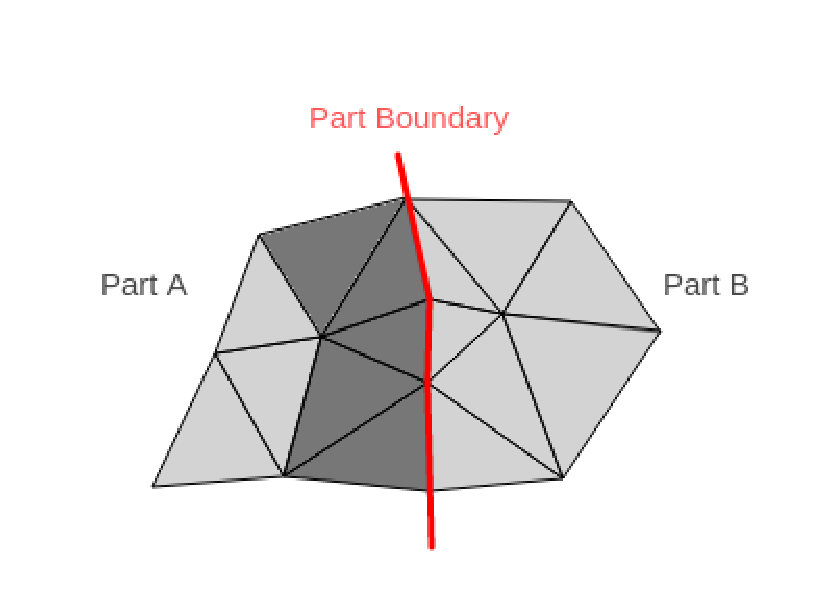
\includegraphics[width=0.8\textwidth]{ghost.eps} 
\caption{\label{fig:ghost3} A layer of ghosted elements from part A to part B. The darker elements represent all the elements on part A that part B will copy to create its remote mesh.}
\end{figure}

ParMA balances the degree-of-freedom holders defined by 
hierarchical Nedelec basis functions~\cite{ko2010advances,ingelstrom2006new} by
reusing existing multi-entity target and boundary-element selection
procedures.
For first order elements this requires balancing edges.
Second order elements requires edges and faces, and above that edges, faces, and
regions need to be balanced.
Each of these entity balancing procedures accounts for the ghosted weight
contribution by performing an additional neighborhood
exchange~\cite{ibanez2014hybrid} of the exact weight of ghosted layer entities.
Thus ParMA can readily account for balancing the work load, in terms of number
of equations per-part, for p-version finite elements by setting mesh entity
weights based on the different entity p-orders.


\section{Fully Parallel In-Memory \dots}
TODO: Ask Cameron/Gerrett To Fill This Out

\section{Adaptive Loop}
At this stage, we have the adaptation loop in place which consists of the following steps:

\setstretch{0.75}
\begin{itemize}
  \item[] while not converged \{
   % \begin{itemize}
	  % \item run SPR to get the size field 
	  % \item \textit{convert 2nd order Lagrange to 2nd order Bezier}
	  % \item \textit{run the curve adapt}
	  % \item \textit{convert 2nd order Bezier back to 2nd order Lagrange}
	  % \item convert the PUMI-mesh to SLAC-mesh for the next solve
	  % \item do a Omega3P solve
	  % \item get the PUMI-mesh with new field values
	  % \item check for convergence
   % \end{itemize}
   %more traditional explanation of the adaptive loop
   \begin{itemize}
          \item partition the mesh with a focus of owned and ghost elements
          \item convert PUMI-mesh to SLAC-mesh
	  \item do a Omega3P solve %could use better wording
	  \item transfer electric field values to the PUMI-mesh
          \item check for convergence
          \item run Super-convergent Patch Recovery (SPR) for error estimation to get the size field
	  \item \textit{convert 2nd order Lagrange to 2nd order Bezier} %not sure if this is really important to them
	  \item \textit{run the curve adapt}
	  \item \textit{convert 2nd order Bezier back to 2nd order Lagrange} %also not sure if important
   \end{itemize}

 \item[] \}
\end{itemize}
\setstretch{1.5}

Figures \ref{pill} and \ref{cav} show two working examples for the curve adaptation loop. 
\begin{landscape}
\begin{figure}[ph!]
\centering
\subfigure[]{\label{pill_init}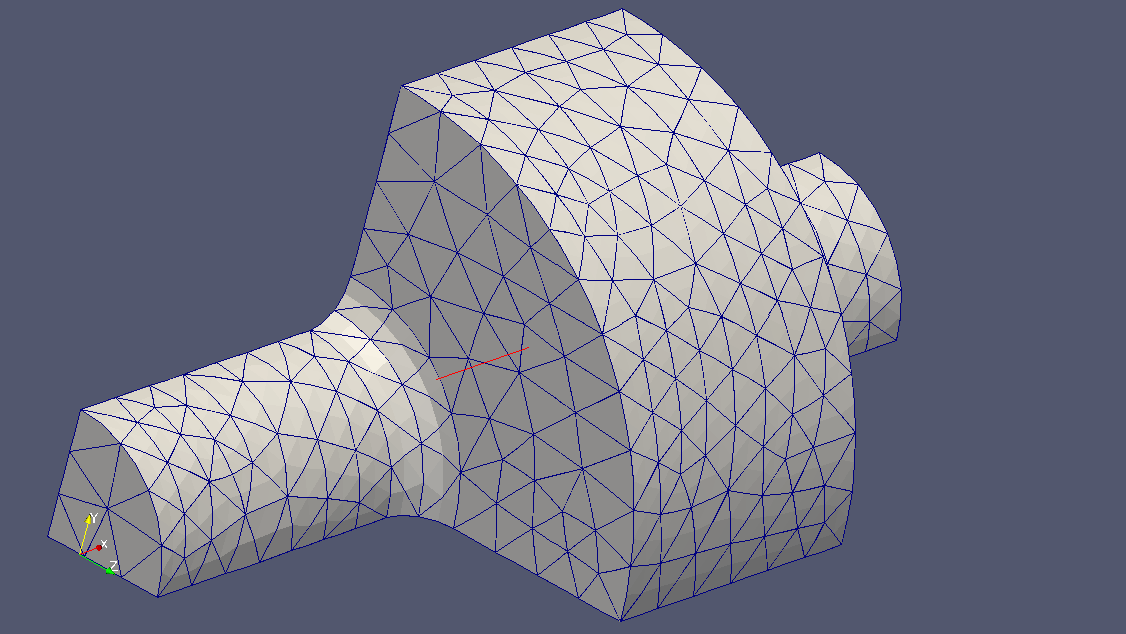
\includegraphics[width=0.55\textwidth]{al_0_ar_0p0125_3721_elems.png}}
\hspace*{50pt}
\subfigure[]{\label{pill_size}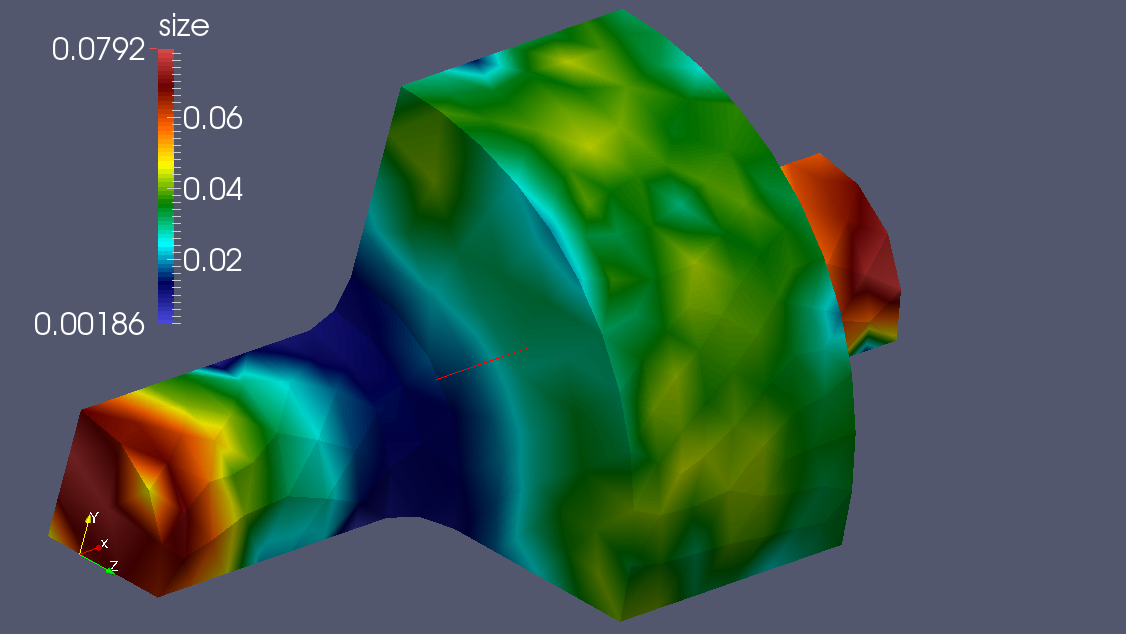
\includegraphics[width=0.55\textwidth]{al_0_ar_0p0125_3721_elems_size_field.png}}
\\
\subfigure[]{\label{pill_adapt}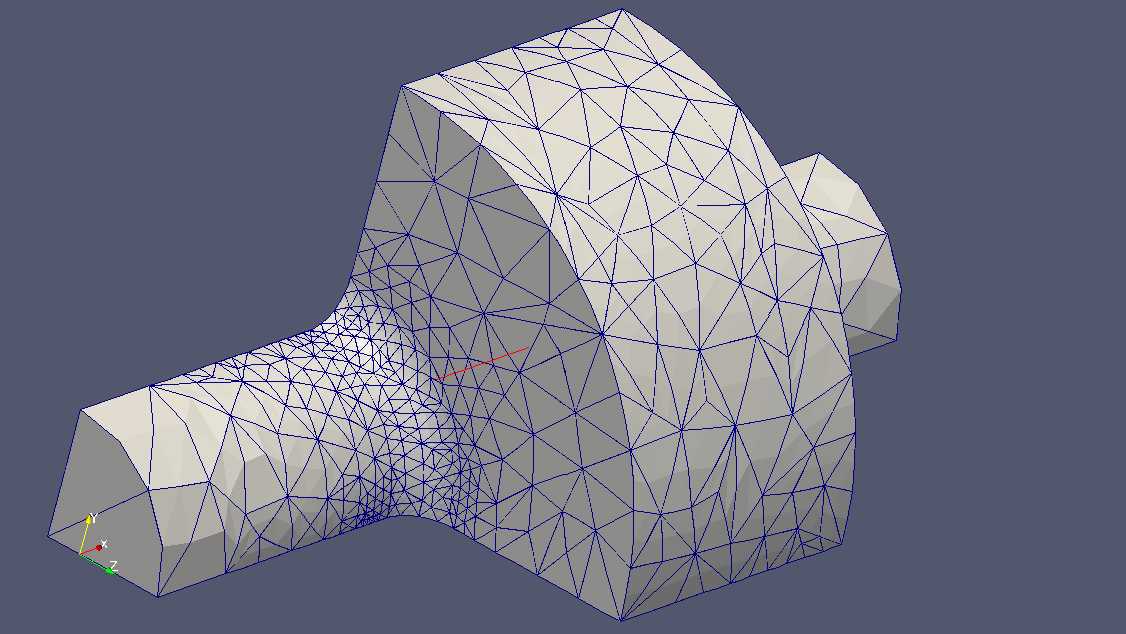
\includegraphics[width=0.55\textwidth]{al_3_ar_0p0125_14221_elems.png}}
\hspace*{50pt}
\subfigure[]{\label{pill_field}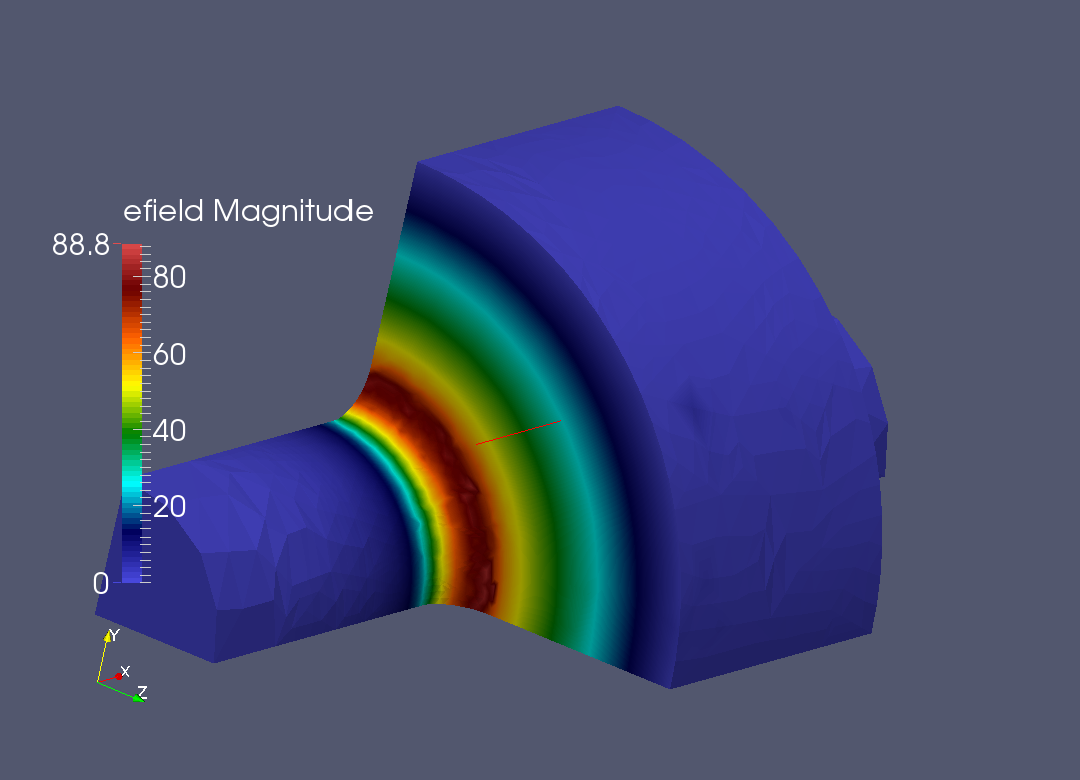
\includegraphics[width=0.55\textwidth]{al_3_ar_0p0125_14221_elems_e_field.png}}
\caption{\label{pill} This Figure shows the results for the PILLBOX model. (a) shows the initial mesh [$\sim3.7\text{K}$ elements], (b) shows the initial size-field, (c) shows the adapted mesh after 3 adaptation steps [$\sim14\text{K}$ elements], and (d) shows the electric field for the final adapted mesh.}
\end{figure}
\end{landscape}
\begin{landscape}
\begin{figure}[ph!]
\centering
\subfigure[]{\label{cav_init}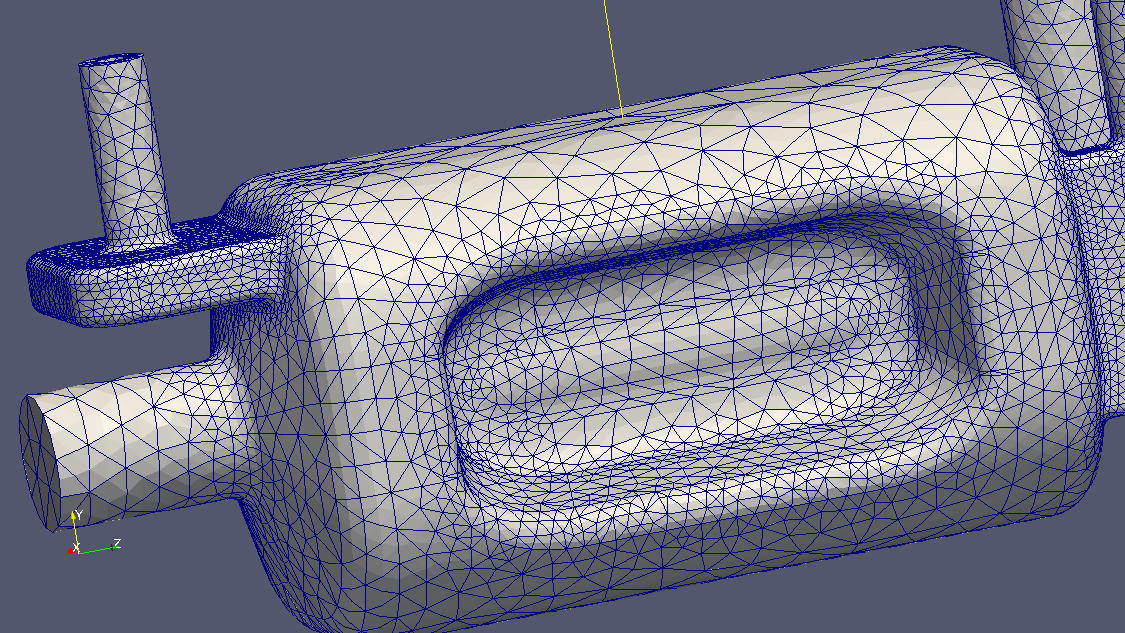
\includegraphics[width=0.55\textwidth]{al_0_ar_0p0125_126044_elems.png}}
\hspace*{50pt}
\subfigure[]{\label{cav_size}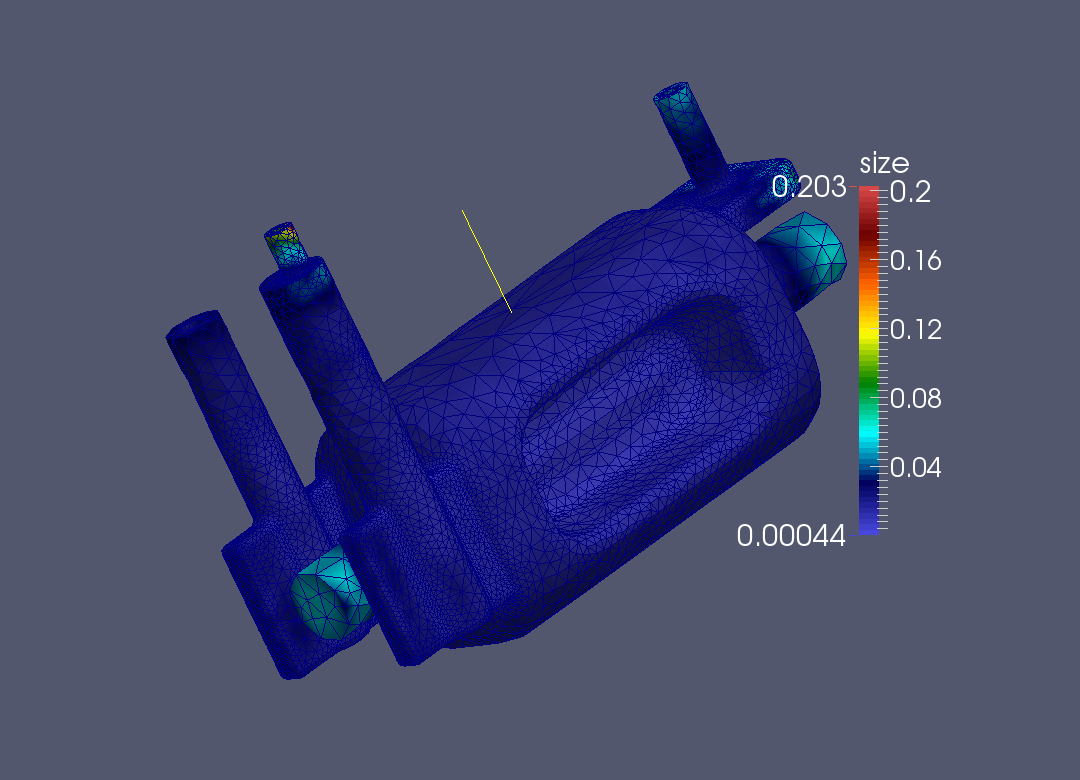
\includegraphics[width=0.55\textwidth]{al_0_ar_0p0125_126044_elems_size_field.png}}
\\
\subfigure[]{\label{cav_adapt}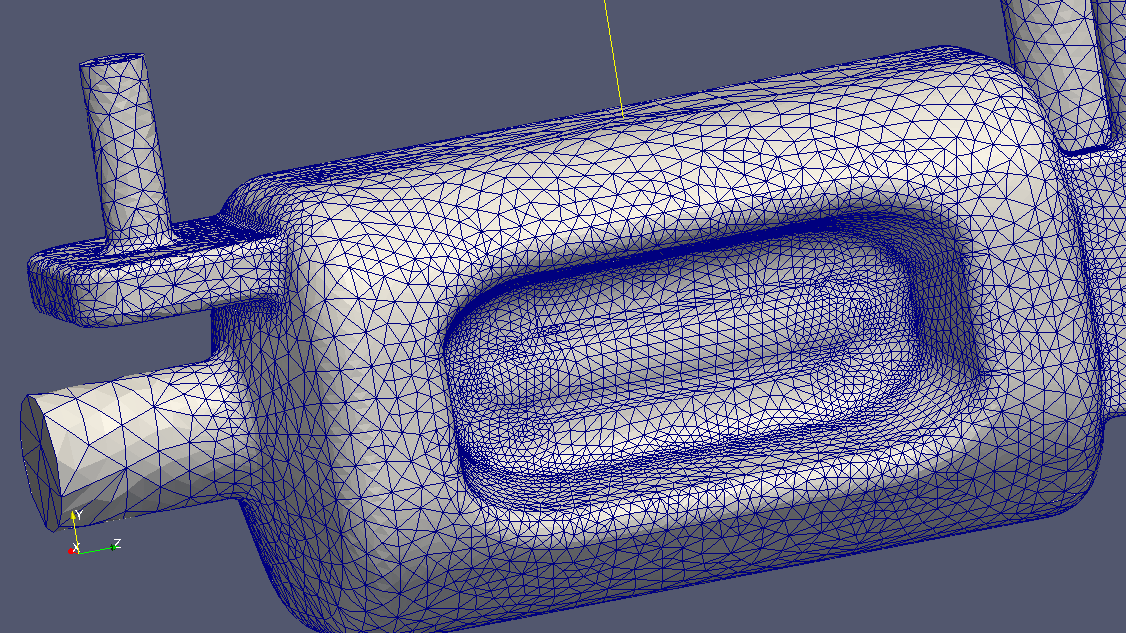
\includegraphics[width=0.55\textwidth]{al_3_ar_0p0125_386896_elems.png}}
\hspace*{50pt}
\subfigure[]{\label{cav_field}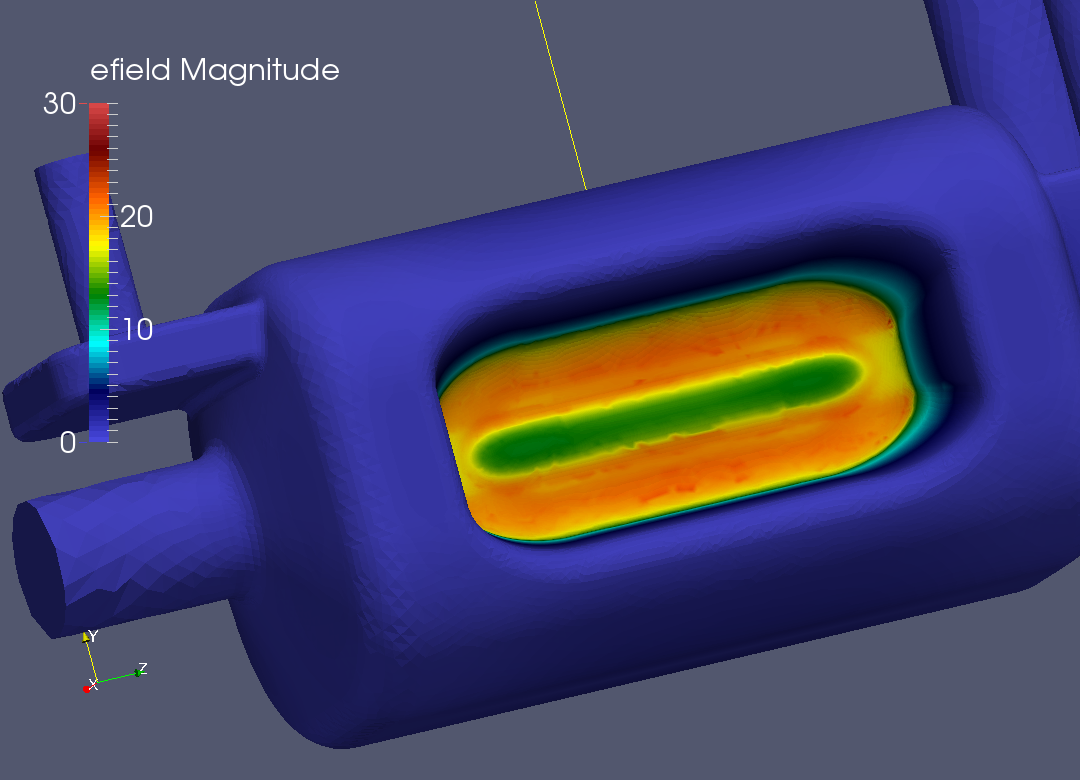
\includegraphics[width=0.55\textwidth]{al_3_ar_0p0125_386896_elems_e_field.png}}
\caption{\label{cav} This Figure shows the results for the CAV17 model. (a) shows the initial mesh [$\sim126\text{K}$ elements], (b) shows the initial size-field, (c) shows the adapted mesh after 3 adaptation steps [$\sim380\text{K}$ elements], and (d) shows the electric field for the final adapted mesh.}
\end{figure}
\end{landscape}
In particular, Fig. \ref{pill} shows the results for the smaller ``PILLBOX''. We start with a uniform and relatively coarse mesh as shown in Fig. \ref{pill_init}. The desired size field for this initial mesh is obtained based on the magnitude of the electric filed and it is shown in Fig. \ref{pill_size}. The final, adapted mesh (for this specific example we needed 3 levels of adaptation) is shown in Fig. \ref{pill_adapt}. Figure \ref{cav} shows the corresponding result for the larger ``CAV17'' model. 


\section{Moving Towards Higher-Order Geometries}
As a first step towards using higher-order geometric elements, we have been able to replace the Omega3P calls to compute determinant of the Jacobian with the corresponding PUMI calls. This is done by storing and additional pointer in each Omega3P-element that points to the corresponding  PUMI-element (see Fig. \ref{imp} for the details of the implementation). 
\begin{figure}[ph!]
\centering
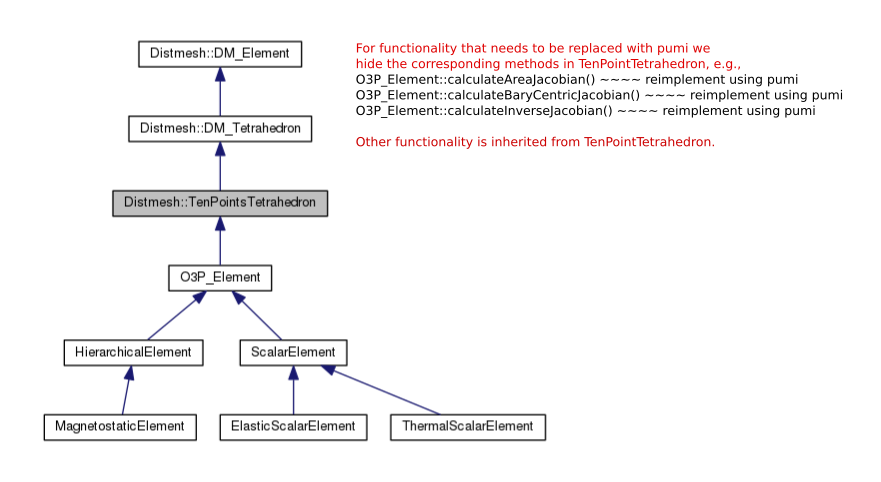
\includegraphics[width=0.95\textwidth]{hide_ten_point_tet.png}
\caption{\label{imp} This Figure shows the implementation details for replacing Omega3P calls for determinant calculation with the corresponding PUMI calls.}
\end{figure}
This, in theory, should make it possible to raise the (geometric) order of the elements. (Currently, we have support for up to 6th order Bezier elements.)

% \section*{References}
% \bibliographystyle{elsarticle-harv_noURL}
% \bibliography{Ref} 

\newpage \bibliographystyle{plain}
\bibliography{scorec-refs/partition,scorec-refs/meshdb,scorec-refs/hardware,scorec-refs/io,scorec-refs/frameworks,scorec-refs/cr,scorec-refs/fem,scorec-refs/meshgen,scorec-refs/msgpass}


\end{document}
